
\section{Generating fractures from surfaces}
To generate a realistic fracture we use the method of successive random additions, as described previously, to generate random surfaces with a known Hurst exponent. We then put one surface above the other, and let the space between the surfaces be the \hl{fracture/void}\footnote{Since we are using periodic systems, we could also have let the space outside the surfaces be the fracture and get the same result. \hl{But for easier visualization.}}.

In practice we make a fractured \hl{silica} structure using the following procedure\hl{:}
\begin{itemize}
    \item Make a liquid SiO$_2$ system.
    \item Generate two surfaces.
    \item Rescale the $(x,y)$-positions of surfaces so they span the size of the system.
    \item Rescale the $z$-values of the surfaces so all points are inside the system.
    \item Remove all atoms between the upper and lower surfaces.
\end{itemize}

Removing all atoms between the two surfaces isn't a trivial task. But since all points in both surfaces lie on a regular grid in the $x$-$y$-plane, there is a simple way of dividing the volume between the surface into tetrahedra, and checking if a point is inside a tetrahedra is a \hl{simple} geometrical exercize that can be solved \hl{programmatically}. If the two surfaces are not intersecting, we see that we can divide the volume between them into convex hexahedra\todo{explain convex hexahedra?}, each spanned out by the points
\begin{align*}
    (x^1_{i}, y^1_{i}), (x^1_{i+1}, y^1_{i}), (x^1_{i}, y^1_{i+1}), (x^1_{i+1}, y^1_{i+1}), \\
    (x^2_{i}, y^2_{i}), (x^2_{i+1}, y^2_{i}), (x^2_{i}, y^2_{i+1}), (x^2_{i+1}, y^2_{i+1}),
\end{align*}
for
\begin{align*}
    0 \leq i,j < N,
\end{align*}
where $(x^1_i,y^1_j)$ are points in one surface and $(x^2_i,y^2_j)$ in the other. We then divide each \hl{convex hexahedra} into five tetrahedron, as illustrated in \cref{fig:hex_to_tetra}, giving a total of $5(N-1)^2$ tetrahedra.
%
% We do this by utilizing the fact that the points in each heighmap lie on a regular grid in the $x$-$y$-plane. This means that we can divide the volume into tetrahedra, . If the two heightmaps are not intersecting, we see that we can divide the volume between them into convex hexahedra, one for each set of points
% ($x_{i}, y_{i}$), ($x_{i}, y_{i+1}$), ($x_{i+1}, y_{i}$), and ($x_{i+1}, y_{i+1}$) 
% % $(x_i, y_i)$  $(x_i, y_{i+1})$ $(x_{i+1}, y_i)$ $(x_{i+1}, y_{i+1})$
% in the $x$-$y$-grid. Each of these hexahedra can then be divided into five tetrahedra, as illustrated in \cref{fig:hex_to_tetra}.
%
% \begin{figure}[htpb]%
%     \centering%
%     
\includegraphics[width=0.4\textwidth]{images/fracture/hexahedron_to_tetrahedra.png}%
%     \caption{%
%         Illustration of how to divide a hexahedron into five tetraheda.%
%         \label{fig:hex_to_tetra}%
%     }%
% \end{figure}%
% %
% \begin{figure}[htpb]%
%     \centering%
%     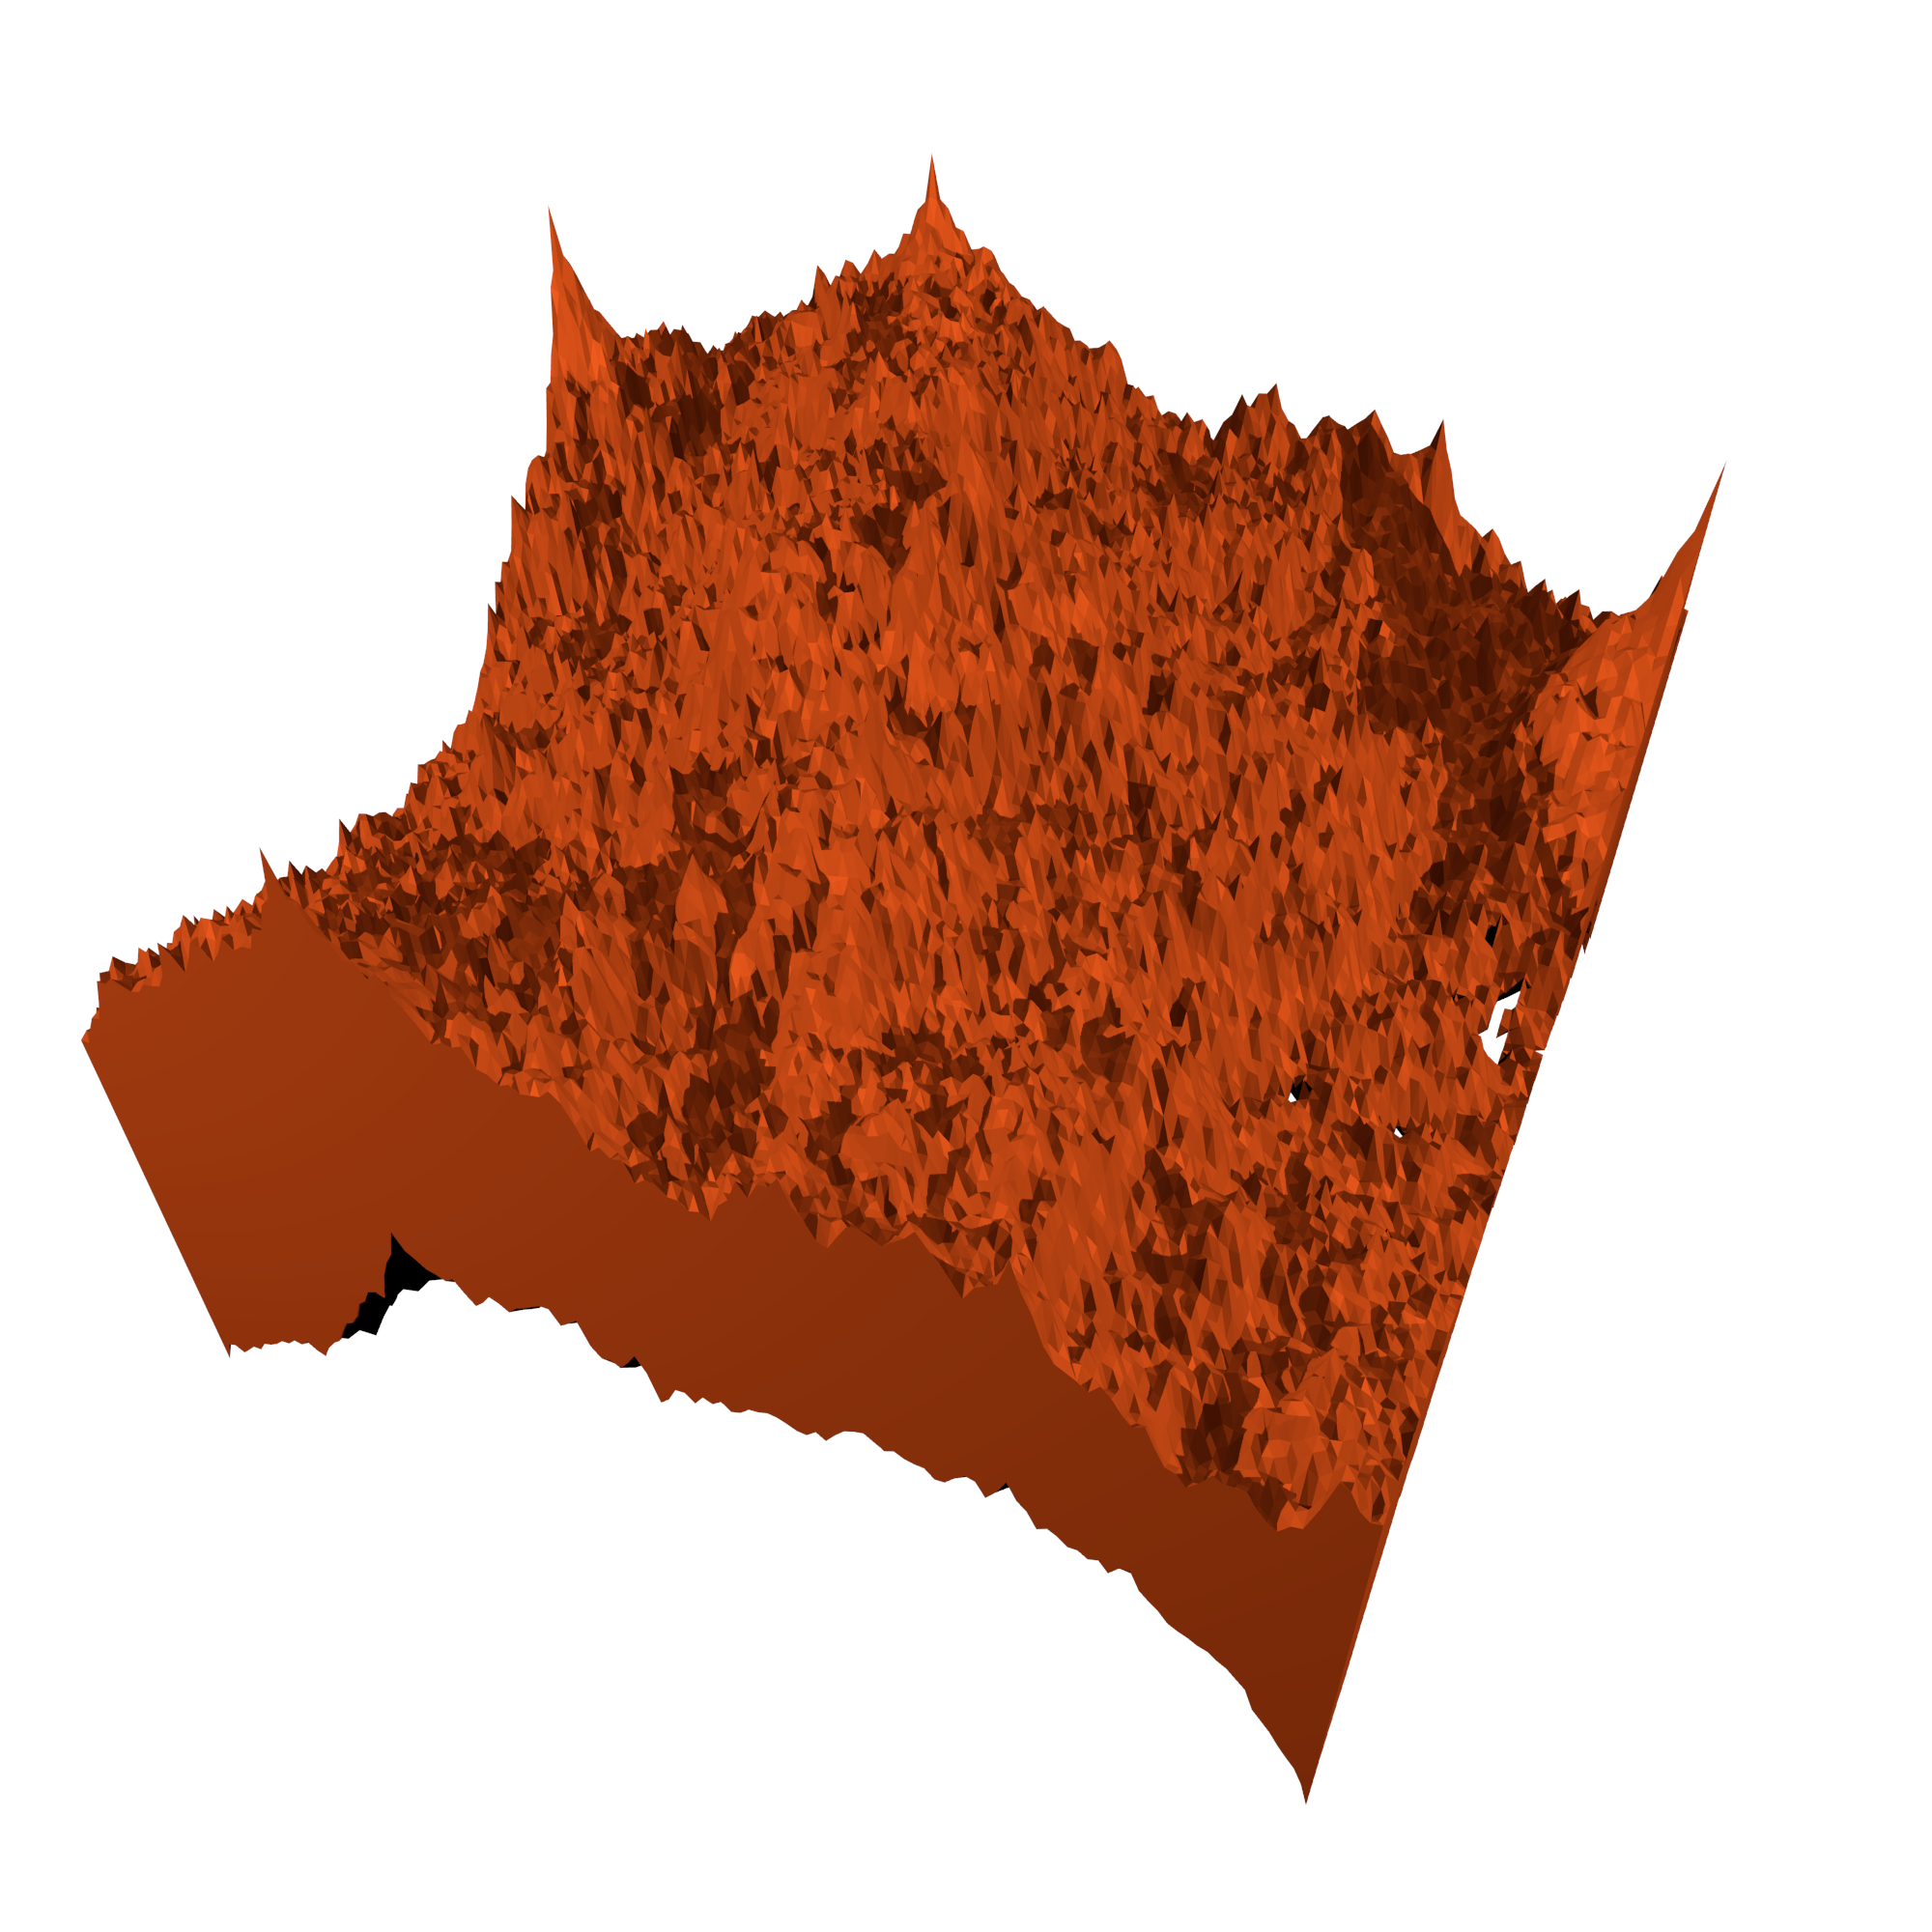
\includegraphics[width=0.6\textwidth]{images/fracture/fracture.png}%
%     \caption{%
%         A model of a fracture.%
%         \label{fig:fracture_model}%
%     }%
% \end{figure}%
%
\begin{figure}[htpb]%
    \centering%
    \setlength{\myfigwidth}{0.4\textwidth}%
%     \setlength{\mycaptionwidth}{0.3\textwidth}%
    \begin{subfigure}[b]{\myfigwidth}%
        \centering% % Need to center to get image centered over caption
        
\includegraphics[width=0.6\textwidth]{images/fracture/hexahedron_to_tetrahedra01_cycles_n200_cropped.png}%
        \caption{Illustration of how to divide a convex hexahedron into five tetraheda.}%
        \label{fig:hex_to_tetra}%
    \end{subfigure}%
    \hspace{0.1\textwidth}%
    \begin{subfigure}[b]{\myfigwidth}%
        \centering%
        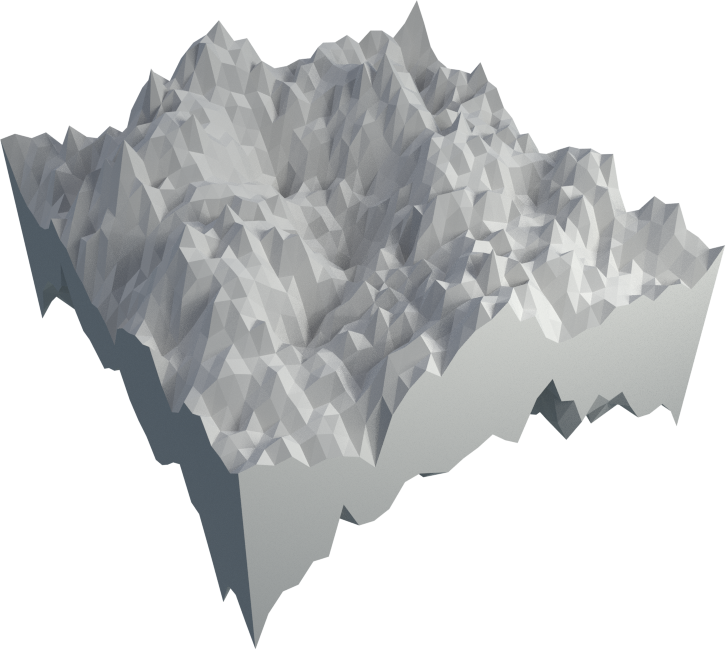
\includegraphics[width=\textwidth]{images/fracture/fracture05_n200_cropped.png}%
%         \includegraphics[width=\textwidth]{images/fracture/large_fracture04_300dpi_w20cm}%
        \caption{A random fracture made from two periodic surfaces.}%
        \label{fig:fracture_model}%
    \end{subfigure}%
\end{figure}%

\subsection{Finding a point inside a tetrahedron}
A tetrahedron consists of four points $\bvec a$, $\bvec b$, $\bvec c$, and $\bvec d$, and four faces spanned by the four possible combinations of the four points. For a face spanned by the points $\bvec a$, $\bvec b$, and $\bvec c$ we can find if a point $\bvec P$ is on the same side of the face as the point $\bvec d$ (the point not used to construct the face) by doing some geometry. We find the normal vector to the surface $\bvec n$ by the cross product 
\begin{align*}
    \bvec n = (\bvec a-\bvec c)(\bvec b-\bvec c).
\end{align*}
We know that the sign of the dot product between this normal vector and another vector going from the plane to a point will give us information about which side of the plane the point is. This means that if two points $\bvec p_1$ and $\bvec p_2$ are on the side of the plane, the dot product between the normal vector and the two vectors
\begin{align*}
    (\bvec p_i - \bvec k),
\end{align*}
where $\bvec k$ is any point in the plane, should have the same sign. So we find the sign of dot products
\begin{align*}
    &\text{sgn}\big(\bvec n\cdot(\bvec P - \bvec k)\big), \\
    &\text{sgn}\big(\bvec n\cdot(\bvec d - \bvec k)\big),
\end{align*}
and if the sign of these dot products is the same, we know that the point $\bvec P$ is on the same side of the face as the point $\bvec d$. We now see that if we do this for all four faces of the tetrahedra, we know that the point $\bvec P$ is inside the tetrahedra if the signs of all pairs of dot products are equal.

% Calculating wether a point is inside a tetrahedron can be reduced to comparing the sign of five different matrix determinants. If we have a point $P = (x,y,z)$ and the four vertices of the tetrahedron are $(x_i, y_i, z_i)$ for $i\in \{1,2,3,4\}$, we can find if the point is inside the tetrahedron by checking if the the following five matrix determinants have the same sign
% \begin{align*}
%     &\begin{vmatrix}
%         x_1 & y_1 & z_1 & 1 \\
%         x_2 & y_2 & z_2 & 1 \\
%         x_3 & y_3 & z_3 & 1 \\
%         x_4 & y_4 & z_4 & 1
%     \end{vmatrix},&
%     &\begin{vmatrix}
%         x & y & z & 1 \\
%         x_2 & y_2 & z_2 & 1 \\
%         x_3 & y_3 & z_3 & 1 \\
%         x_4 & y_4 & z_4 & 1
%     \end{vmatrix},&
%     &\begin{vmatrix}
%         x_1 & y_1 & z_1 & 1 \\
%         x & y & z & 1 \\
%         x_3 & y_3 & z_3 & 1 \\
%         x_4 & y_4 & z_4 & 1
%     \end{vmatrix},&
%     \\
% %     \vspace{5mm}
%     \\
%     &\begin{vmatrix}
%         x_1 & y_1 & z_1 & 1 \\
%         x_2 & y_2 & z_2 & 1 \\
%         x & y & z & 1 \\
%         x_4 & y_4 & z_4 & 1
%     \end{vmatrix},&
%     &\begin{vmatrix}
%         x_1 & y_1 & z_1 & 1 \\
%         x_2 & y_2 & z_2 & 1 \\
%         x_3 & y_3 & z_3 & 1 \\
%         x & y & z & 1
%     \end{vmatrix}.&
% \end{align*}
